% siminos/marginal/marginal.tex
% $Author: predrag $ $Date: 2019-04-20 19:07:04 -0400 (Sat, 20 Apr 2019) $

%\svnkwsave{$RepoFile: DOGS/marginal/marginal.tex $}
%\svnidlong {$HeadURL: svn://zero.physics.gatech.edu/siminos/blog/marginal.tex $}
%{$LastChangedDate: 2019-04-20 19:07:04 -0400 (Sat, 20 Apr 2019) $}
%{$LastChangedRevision: 6840 $} {$LastChangedBy: predrag $}
%\svnid{$Id: marginal.tex 6840 2019-04-20 23:07:04Z predrag $}

\chapter{The meaning of it all}
\label{c-marginal}
% Predrag started the writeup 2013-08-08

\newcommand{\turbulence}{shmurbulence}

\PC{2013-08-08 Predrag  0.1  attempt to explain the inertial manifold as
        a set nearly marginal, entangled modes; towards a paper with cardiac
        folks. But it was impossible to write it - first they did not understood
        me, later at least one of them assume he understood it first, so there was
        no point of putting my name on ``their'' paper.}

% clipped from pipes/focusPOT/focusPOT.tex:
Turbulent flows never settle down, yet we can recognize a cloud by its
transitory shapes. What are these fleeting shadows? The discovery of
unstable steady and travelling solutions of Navier-Stokes equations,
together with glimpses of them in experiments\rf{science04}, carries a
promise of obtaining a description of a turbulent flow in terms of the
dynamics of a handful of exact solutions. Intriguing as they are, these
solutions are shapes that do not change in time. However, turbulence
does, and to capture it one needs dynamics.

% clipped from pipes/focusPOT/focusPOT.tex:
The possibility that one could
adjust the myriad of initial velocity fields of a 3$D$ turbulent fluid
state in such a way that the flow would \emph{exactly} recur after a
finite time had always seemed utterly out of reach.
That is, until the Christmas of 2000, when Kawahara and Kida\rf{KawKida01} announced
that they had found an ``unstable periodic solution of the
Navier-Stokes equation,'' in a 8,448\dmn\ discretization of the \pCf!
This solution was not only periodic in time, but lay smack in the
turbulent sea and predicted turbulent averages surprisingly well.
Once the first transistor is built, the impossible becomes possible,
and heroic feat that it was, it was eventually followed by
several groups\rf{Visw07b,CviGib10,KreEck12,ACHKW11},
who have so far determined some hundred such solutions for 3$D$ flows.
Today, an undergraduate can download
\HREF{http://www.channelflow.org/} {Channelflow.org} code and find
even more. A single solution makes for a pretty journal cover. But
an infinity of orbits...

% clipped from pipes/focusPOT/focusPOT.tex:
Chandler and Kerswell\rf{ChaKer12} (C\&K) have undertaken the most exhaustive
study so far of periodic orbit theory (POT) applied to fluid
dynamics.
\Po s are one class of invariant solutions (acronym UPOs for
Unstable Periodic Orbits is also used, a bit like calling all
bicycles `unstable bicycles'). C\&K `\recFlow' is broader and more
descriptive of the plethora of invariant solutions encountered in
fluid dynamics: `coherent structures', `recurrent patterns',
`modulated amplitude waves', and so on. C\&K investigate
2$D$ Kolmogorov flow on a doubly periodic domain at several
moderate Reynolds numbers, resolved to 22,428 degrees of freedom. An
individual turbulent state tends to break all symmetries, so searches
are undertaken in the full \statesp, with no symmetry restrictions.
First, DNS simulations are run
for long times. Near recurrences are flagged and used as
starting guesses for \recFlow s,  which are then determined by an
iterative Newton-Raphson root search; their linear stability is
computed by the Arnoldi method. After CPU months of trawling, some
hundred \recFlow s are determined, typically with 4-5 unstable
eigen\-directions. \RecFlow s are
profitably viewed as videos; see the \texttt{Channelflow.org}
\HREF{http://channelflow.org/dokuwiki/doku.php?id=database} {data
base}. Embedded in the turbulent flow, these solutions are likely to
be dynamically important.

Consider a dissipative spatiotemporal dynamical system described by some
nonlinear PDE.

First, there is typically a `quiescent', `laminar', etc., \eqv\
solution that the flow settles into in the high viscosity limit. Due to its
high symmetry, we can often compute analytically the full spectrum of its
linearized perturbation eigenmodes and eigenvalues
(Orr-Sommerfeld eigenfunctions\rf{OK96,Coff76}, Squire modes, Stokes modes, ...).
    \PC{2007-02-18 - %gibson/blog/UBLBfeb07/from ublbfeb07.tex
Panton\rf{Pan96}, Sect 22.3: Squire's theorem\rf{Sq33} shows that for any
3\dmn\ disturbance there is a corresponding 2\dmn\ disturbance that is
more unstable. I interpreted to mean that the more constrained a solution is, the more unstable it
is. For example, the simplest solutions within a symmetry invariant subspace are
more unstable than comparable solutions in the full \statesp.
    }
For \KS\ these
are simply the Fourier modes. For a given viscosity, certain number of the
long wavelength modes are unstable, while the high wavelength modes
are always damped by the viscosity. If we double the outer length scale $L$
of the system, the number of unstable modes will double.
    \PC{be more explicit!}

The thing about very unstable invariant solutions is that there is no
dynamical path to make them recurrent, even if a symmetry imposes a
heteroclinic connection to them. As an example, we have worked in detail
the `quiescent' Lorenz system \eqv\ solution $(x,y,z)=(0,0,0)$ in
\HREF{http://www.streamsound.dk/book1/chaos/chaos.html\#111/z}
{Example 4.7} {\em Stability of Lorenz flow
equilibria}; it is impossible for the flow to revisit the
neighborhood of that \eqv. So while applied mathematicians might love
such solutions and the bifurcations therefrom, no turbulent dynamics
takes place there.

Now, assume that there is typical spatial length scale $\ell$ in the problem.
For \KS\ this scale is determined by the balance of the Laplacian with
wrong sign (that injects energy into the flow rather than damping it),
{\em vs.} the hyper diffusion (Laplacian squared) that strongly
suppresses high wave numbers. For 2D spiral chaos this length scale is
the Gaussian width of a spiral core. For a 3D boundary shear fluid flow
it is the local width of the viscous boundary layer, or a geometrical
scale, such as the wall-to-wall distance or the pipe diameter.

Cells just large to fit two-three such scales suffice to exhibit a finite
number of unstable \eqv\ and \reqv\ solutions, and the usual exponential infinity
of \po s and \rpo s. For \KS\ we have more than 50,000 such solutions\rf{SCD07}.

\section{Slice \& dice}
\label{s:SliceDice}

For a single core, which, unless you are working in a discrete symmetry
subspace, is a \reqv, I assume that in the computation you are
implementing the three slice conditions that eliminate the overall
continuous symmetries, as was described here
-but youtu.be/qtccix8Dhok is no more- (in case of a \rpo\ one would also need a
section, as discussed here \YTlink{youtu.be/wUbkYPsjVnc}).

For two or more localized, well separated cores, the marginal
eigenvectors identify which core is drifting
\YTlink{youtu.be/KCP3twrHb5Y}. I recommend dicing
\YTlink{youtu.be/zZ9FF4jqV-U}.

%%%%%%%%%%%%%%%% start ChaosBook inset %%%%%%%%%%%%%%%%%%%%%%%%%%%%
\section{Symmetries of solutions}
\label{s:contSymmSol}
% from ChaosBook \Chapter{continuous}{Relativity for cyclists}
% Predrag                                  19may2013

        \index{symmetry!solution}
        \index{solution!symmetry}

Let $\vel(\ssp)$ be the dynamical flow, and $f^\tau$ the
trajectory or  `time-$\tau$ forward map' of an initial point
$\xInit$,
    \index{time-$t$ forward map}
\beq
\frac{d\ssp}{dt} = \vel(\ssp)
    \,, \qquad
    \ssp(\tau) = f^\tau(\xInit)
        = \xInit + \int_0^\tau \! d \tau'\,  \vel(\ssp(\tau'))
\,.
\label{symbolicNS}
\eeq
Solutions $\ssp(\tau)$
of an equivariant system can satisfy all of
the system's symmetries, a subgroup of them, or
have no symmetry at all. For a given solution $\ssp(\tau)$, the
subgroup that contains all symmetries that fix $\ssp$ (that satisfy
$\LieEl \ssp = \ssp$) is called the isotropy (or stabilizer) subgroup of $\ssp$.
A generic
ergodic trajectory $\ssp(\tau)$ has no symmetry beyond the identity,
so its isotropy group is $\{e\}$,
but recurrent solutions often do. At the other extreme is
{\eqv}, whose isotropy group is the full symmetry
group $\Group$.

The  simplest solutions are the {\em \eqva} or {\em steady}
solutions.

\paragraph{Definition:
           \Eqv}
            \index{equilibrium}
$\ssp_{\EQV{}} = \pS_{\EQV{}}$ is a fixed,
time-invariant solution,
\bea
\vel(\ssp_{\EQV{}}) &=& 0  \,,
    \continue
 \ssp(\ssp_{\EQV{}},\tau)
      &=& \ssp_{\EQV{}} + \int_0^\tau \! d \tau'\,  \vel(\ssp(\tau'))
       =  \ssp_{\EQV{}}
\,.
\label{eq:eqva}
\eea
An {\em \eqv} with full symmetry,
\index{group!orbit}\index{orbit!group}
\[
\LieEl \, \ssp_{\EQV{}}=\ssp_{\EQV{}}
    \qquad \mbox{ for all } \LieEl \in \Group
\,,
\]
lies, by definition,  in $\Fix{\Group}$ subspace. The multiplicity of such solution is
one. An {\eqv} $\ssp_{\EQV{}}$ with symmetry $\stab{\EQV{}}$ smaller than
the full group $\Group$ belongs to a group orbit $\Group/\stab{\EQV{}}$.
If $\Group$ is finite there are $|\Group|/|\stab{\EQV{}}|$ \eqva\ in the
group orbit, and if $\Group$ is continuous then the group orbit of $\ssp$
is a continuous family of \eqva\ of dimension $\dim \Group - \dim
\stab{\EQV{}}$. For example, if the angular velocity $\velRel$ equals
zero, the group orbit consists of a circle of (dynamically static)
equivalent \eqva.

\paragraph{Definition:
           \Reqv}
            \index{relative!equilibrium}
            \index{equilibrium!relative}
solution  $\ssp_{\REQV{}{}}(\tau) \in \pS_{\REQV{}{}}$:
the dynamical flow field points
along the group tangent field, with constant
`angular' velocity  \velRel, and the trajectory stays on the
group orbit:
\bea
\vel(\ssp) &=& \velRel \cdot \groupTan(\ssp)
    \,,\qquad
               \ssp \in \pS_{\REQV{}{}}
    \continue
\ssp(\tau)  &=& \LieEl(-\tau \, \velRel) \, \ssp(0)
   \,=\,
   e^{-\tau \, \velRel \cdot \Lg} \ssp(0)
    \,.
\label{contInvSolns}
\eea
A  {\em traveling wave}
\index{traveling wave}\index{rotating wave}
\beq
\ssp(\tau)   =  \LieEl(-\velRel \tau) \, \ssp_{\REQV{}{}}
  = \ssp_{\REQV{}{}} - \velRel \, \tau \,,\quad  \velRel \in \reals^d
\ee{BeThTW}
is a special type of
a \reqv\ of equivariant evolution equations,
where the action is given by translation,
$ %\beq
\LieEl(y) \, \ssp(0)
  = \ssp(0) + y
\,.
$ %\ee{BeThTW}
A {\em rotating wave} is another special case of \reqv,
with the action is given by angular rotation.
By equivariance, all points on the group orbit are equivalent,
the magnitude of
the velocity $\velRel $ is same everywhere along the
orbit, so a `traveling wave' moves at a constant speed.
For an $N>1$ trajectory traces out a line within the
group orbit. As the $\velRel_a $ components are generically not in
rational ratios, the trajectory explores the
$N$-dim\-ens\-ion\-al group orbit
quasi-periodically. In other words, the group orbit
$\LieEl(\tau) \, \ssp(0)$ coincides with the dynamical orbit
$\ssp(\tau) \in \pS_{\REQV{}{}}$ and is thus flow invariant.

\paragraph{Definition:
           \Po.}
           \index{periodic!orbit}
Let $\ssp$ be a periodic point on the \po\ $p$ of period
$\period{}$,
\[
f^\period{}(\ssp) = \ssp
    \,,\qquad
\ssp \in \pS_p.
\]
By equivariance, $\LieEl \, \ssp$ is another periodic point,
with the orbits of $\ssp$ and $\LieEl \ssp$ either identical
or disjoint.

If $\LieEl \ssp$ lands on the same orbit,  $\LieEl$ is
an element of periodic orbit's symmetry group
$\stab{p}$. If the symmetry  group is the full
group $\Group$, we are back to \refeq{contInvSolns}, \ie,
the periodic orbit is the group orbit traced out by a \reqv.
The other option is that the isotropy group is discrete,
the orbit segment $\{\ssp,\LieEl \ssp\}$
is pre-periodic (or eventually periodic),
$\ssp(0)= \LieEl_p  \ssp(\period{p})$, where $\period{p}$ is a fraction
 of the full period, $\period{p}=\period{}/m$, and thus
\bea
	\ssp(0) &=& \LieEl_p \ssp(\period{p})
\,,\qquad
    \ssp \in \pS_p
\,,\qquad
	\LieEl_p \in \stab{p}
\continue
	\ssp(0) &=& \LieEl_p^m \ssp(m \, \period{p})
                      = \ssp(\period{}) =  \ssp(0)
\,.
\label{preperiodic}
\eea

If the periodic solutions are disjoint,
their multiplicity (if $\Group$ is
finite), or the dimension of the
manifold swept under the group action (if $\Group$ is
continuous) can be determined by applications of $\LieEl \in
\Group$. They form a family of conjugate solutions,
\beq
	\pS_{\LieEl\, p}=\LieEl\, \pS_p \, \LieEl^{-1}\,.
\ee{cont:conjIsotr}

\paragraph{Definition:
           \Rpo}
$p$ is an orbit $\pS_p$ in {\statesp} $\pS$
which exactly recurs
    \index{periodic!orbit!relative}\index{relative!periodic orbit}
    \index{period!relative}\index{relative!period}
\beq
\ssp_p (0) = \LieEl_p \ssp_p (\period{p} )
    \,,\qquad
\ssp_p (\tau) \in \pS_p
    \,,
\label{RPOrelper1}
\eeq
at a fixed {\em relative period} $\period{p}$, but
shifted by a fixed group action ${\LieEl_p}$
which brings the endpoint $\ssp_p (\period{p} ) $
back into the initial point $\ssp_p (0) $.
The group action ${\LieEl_p}$ parameters
$\gSpace = (\gSpace_1,\gSpace_2,\cdots\gSpace_N)$
are referred to as ``phases,'' or ``shifts.''
%
In contrast to the pre-periodic \refeq{preperiodic}, the
phase here are irrational, and the trajectory sweeps out
ergodically the group orbit without ever closing into a \po.
For dynamical systems with only continuous (no discrete)
symmetries, the parameters $\{t,\gSpace_1,\cdots,\gSpace_N\}$
are real numbers, ratios $\pi/\gSpace_j$ are almost never
rational, likelihood of finding a {\po} for such system is
{zero}, and such \rpo s are almost never eventually periodic.


\Rpo s are to periodic solutions what \reqva\ (traveling
waves) are to \eqva\ (steady solutions). \Eqva\ satisfy
$f^\tau(\ssp) - \ssp = 0$ and \reqva\ satisfy $f^\tau(\ssp) -
\LieEl( \tau) \, \ssp= 0$ for any $\tau$. In a co-moving
frame, \ie, frame moving along the group orbit with velocity
$\vel(\ssp) = \velRel \cdot \groupTan(\ssp)$, the \reqv\
appears as an \eqv. Similarly, a {\rpo} is periodic in its
mean velocity $\velRel_p=\gSpace_p/\period{p}$ co-moving
frame, but in the
stationary frame its trajectory is quasiperiodic. A co-moving
frame is helpful in visualizing a single `relative' orbit,
but useless for viewing collections of orbits, as each one
drifts with its own angular velocity. Visualization of all
\rpo s as \po s we attain only by global symmetry reductions.

%%%%%%%%%%%%%%%% end ChaosBook inset %%%%%%%%%%%%%%%%%%%%%%%%%%%%

\section{Stability of solutions}
\label{s:StabSols}

Multipliers of Jacobian matrices are natural for discrete time maps,  rates (eigen-exponents per unit time) are natural for continuous time flows. An example of linear stability spectrum for flows is \HREF{http://chaosbook.org/tutorials/eqbaStab.html} {here}.

\subsection{Instantaneous rate of shear}

The system of linear {\em equations of variations}
for the displacement of the infinitesimally close neighbor
$\ssp+\deltaX$
follows from
the flow equations \refeq{odes} by Taylor expanding to linear order
\[
\dot{\ssp}_i + \dot{\deltaX}_i =
    \vel_i( \ssp+\deltaX) \approx
    \vel_i(\ssp) + \sum_j {\pde \vel_i \over \pde \ssp_j} \deltaX_j
\, .
\]
The infinitesimal displacement $\deltaX$ is thus transported along the
trajectory $\ssp(\xInit,t)$, with time variation given by
\index{equations of variations}
\beq
{d \over dt} \deltaX_i(\xInit,t) =
\sum_j \left.{\pde \vel_i  \over \pde \ssp_j}(\ssp)
       \right|_{\ssp=\ssp(\xInit,t)}
         \deltaX_j(\xInit,t)
\, .
\label{lin_odes}
\eeq
As both the displacement and the trajectory depend on the initial
point $\xInit$ and the time $t$, we shall often abbreviate the
notation to
$\ssp(\xInit,t) \to \ssp(\zeit) \to \ssp$,
$\deltaX_i(\xInit,t) \to \deltaX_i(t) \to \deltaX$
in what follows. Taken together, the set of equations
\beq
\dot{\ssp}_i={\vel}_i(\ssp) \,, \quad
\dot{\deltaX}_i= \sum_j {\Mvar}_{ij}(\ssp){\deltaX }_j
% \qquad\mbox{where~}\,\, {\Mvar}_{ij}(\ssp) =\pde_j v_i(\ssp)\, .
\ee{die}
governs the dynamics in the tangent bundle
$(\ssp,\deltaX) \in  {\bf T}\pS$
\PC{fix notation: ${\bf(T)}\pS$?}
obtained by adjoining the $d$-dim\-ens\-ion\-al
% fiber, the
tangent space
$\deltaX \in T\pS_{\ssp}$
to every point $\ssp\in \pS$ in the $d$-dim\-ens\-ion\-al {\statesp}
$\pS \subset  \reals^{d}$.
The {\em \stabmat} (\velgradmat)
\index{tangent!space}
\index{tangent!bundle}
\index{matrix!stability}
\index{stability!matrix}
\index{velocity gradients matrix}
\PC{
is it worth defining here the Cartesian decomposition
into symmetric stretching matrix (volume, shape changes)
$
{\bf D} = (\Mvar + \transp{\Mvar})/2
$
and antisymmetric spin matrix (rigid body rotations)
$
{\bf \Omega} = (\Mvar - \transp{\Mvar})/2
$?
   }
\beq
{\Mvar}_{ij}(\ssp) ={\pde \vel_i(\ssp)\over \pde \ssp_j  }
\ee{DerMatrix}
describes the instantaneous rate of shearing of the infinitesimal
neighborhood of $\ssp(\zeit)$
by the flow.


\section{Karma 1994 model}
\label{s:Karma1994}


% \item[2013-06-18 Predrag]
%
I need to know more precisely what is it that Chris is
simulating, so for my own education here I'll clip and paste here
from \textbf{2012-01-29 LS} Luis's \texttt{DOGS/saldana/lit.tex}
notes on Karma\rf{Karma1994}
{\em Electrical alternans and spiral wave breakup in cardiac
tissue}. (I put a copy into the ChaosBook.org/library,
\HREF{http://ChaosBook.org/library/Karma1994.pdf}{click here}.)
All equations and tables are taken from Karma 1994 paper unless
stated otherwise. The Karma 1994 model is:
\bea
\frac{\partial E}{\partial t} &=& \gamma\nabla^{2}E+\tau_{E}^{-1}f(E,n)
    \continue
\frac{\partial n}{\partial t}&=&\tau_{n}^{-1}g(E,n)
    \continue
f(E,n)&=&-E+[E^{*}-\mathcal{D}(n)]h(E)
    \continue
g(E,n)&=&\mathcal{R}(n)\Theta(E-E_n)-[1-\Theta(E-E_n)]n
\,,
\label{eq:Karma1994}
\eea
where $\Theta(x)$ is the Heaviside step function, $E$ is a
dimensionless representation of the trans-membrane voltage, and the
variable $n$ plays the role of a slow current gate variable. The rest
state of the membrane corresponds to $E=n=0$. $E_n$ and $E^*$ are
constants (see Table I) and $h(E)$ is the function
\beq
h(E)=\frac{E^2}{2}[1-\tanh(E-E_h)]
\,,
\ee{eq:Karma1994a}
chosen so that the first model
equation has two stable fixed points corresponding to depolarized and
repolarized states of the membrane. In order to completely determine
the equations of the model, the restitution function $\mathcal{R}(n)$
and the dispersion function $\mathcal{D}(n)$ need to be specified. In
general, it is possible to choose both functions to fit arbitrary
restitution and dispersion curves. The relative abruptness of
excitation is controlled by the parameter $\epsilon=\tau_E/\tau_n$
which is small in the physiological relevant limit of the model.

In the small $\epsilon$ limit, $\mathcal{R}(n)$ is uniquely related
to the restitution curve $A(D)$ ($A(0)=0$) via Eq.~(6) with $A$ the
action potential duration immediately following a diastolic interval
$D$. Karma chooses Eq.~(7) as a simple form for $\mathcal{R}(n)$
which leads to the restitution curve of Eq.~(8). With this form of
$A(D)$, the restitution properties of the tissue are controlled by
the parameter $Re$. Increasing $Re$ increases the steepness of the
restitution curve at short $D$ which renders the tissue more
susceptible to alternans. The slope $S$ of the restitution curve is a
measure of this steepness. For small $\epsilon$, $S=\exp{Re}-1$ and
$Re$ is proportional to the maximum action potential duration
$A_{max}$ in this limit. Also, for small $\epsilon$, $\mathcal{D}(n)$
is uniquely related to the dispersion curve via Eq.~(11) where $c(D)$
is the pulse speed and $C(X)$ (dimensionless) is fitted by a
polynomial numerically calculated for specific $h(E)$. Karma uses the
simple form $\mathcal{D}(n)=n^M$ where $M$ controls dispersion;
larger $M$ leads to weaker dispersion. A stability criterion
previously derived by
Nolasco and Dahlen\rf{Nolasco1968} states that having a slope
of the restitution curve greater than unity for a certain period
leads to alternans. This criterion is exact in the small $\epsilon$
limit of the model. Furthermore, the expression for the minimum
stimulation period $T_{min}$ below which the action potential
duration alternates is given by Eq.~(14).





% siminos/marginal/marginalAckn.tex
% $Author: predrag $ $Date: 2019-04-20 19:07:04 -0400 (Sat, 20 Apr 2019) $

%\svnkwsave{$RepoFile: DOGS/marginal/ackn.tex $}
%\svnidlong {$HeadURL: svn://zero.physics.gatech.edu/siminos/blog/marginalAckn.tex $}
%{$LastChangedDate: 2019-04-20 19:07:04 -0400 (Sat, 20 Apr 2019) $}
%{$LastChangedRevision: 6840 $} {$LastChangedBy: predrag $}
%\svnid{$Id: marginalAckn.tex 6840 2019-04-20 23:07:04Z predrag $}

\bigskip
\noindent {\bf Acknowledgments.}
This report is inspired by the C.~Marcotte and G.~Byrne numerical
studies of spiral chaos in cardiac dynamics, D.~Barkley, M.~Avila and B.~Hof
work on transition to turbulence for pipes and planes,
J.~Gibson, T.~Schneider and J.~Burke's snaking, F.~Ginelli and friends'
numerical computations of covariant vectors for PDE attractors,
R.~Grigoriev's dark and misleading
hints as to the role of ``local gauge invariance''
in systems whose equations (but not boundary conditions) exhibit
continuous invariance, and
 interactions with
[...] and
[...] .
P.C. thanks late Glen Robinson Jr. for support. 	

\newpage

\section{Predrag's blog}
\label{s:blogPC}

%%%%%%%%%%%%%%%%%%%%%%%%%%%%%%%%%%%%%%%%%%%%%%%%%%%%%%%%%%%%%%%%%%%%%
\begin{figure}
   \centering
  \setlength{\unitlength}{0.80\textwidth}
  \begin{picture}(1,0.64588119)%
    \put(0,0){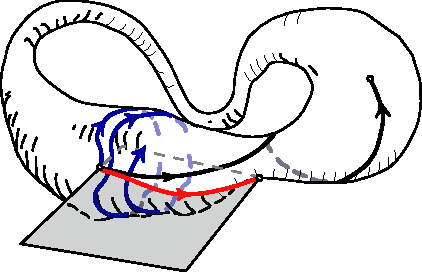
\includegraphics[width=\unitlength]{A29sliceCoMov}}%
    \put(0.06512945,0.38743919){\color[rgb]{0,0,0}\makebox(0,0)[lb]{\smash{$p$}}}%
    \put(0.13158095,0.26355825){\color[rgb]{0,0,0}\makebox(0,0)[lb]{\smash{$\ssp(0)$}}}%
    \put(0.8928881,0.49773156){\color[rgb]{0,0,0}\makebox(0,0)[lb]{\smash{$\bar{\ssp}(\zeit)$}}}%
    \put(0.60833654,0.17543348){\color[rgb]{0,0,0}\makebox(0,0)[lb]{\smash{$\sspRed(\zeit)$}}}%
    \put(0.35487098,0.31486014){\color[rgb]{0,0,0}\makebox(0,0)[lb]{\smash{$\ssp(\zeit)$}}}%
  \end{picture}%
   \caption{\label{fig:A29sliceCoMov}
A \reqv\ is a trajectory which lies in its group orbit, with
$\vel(\ssp)$ in the group tangent space of $\ssp$. For any \SOn{2}
example, it is a 1\dmn\ loop, as in \refeq{fig:A27wurst}\,(b). A
generic trajectory is a {\wurst}, a 2\dmn\ nonlinearly contorted tube
traced out by a combination of a `rotation' in the symmetry
direction, and a strictly non-zero component of $\vel(\ssp(\zeit))$
outside the group tangent space, leading to a time evolving
`shape-changing' dynamics. If one picks a starting point $\ssp(0)$
close to a \reqv\ orbit, the velocity $\vel(\ssp)$ along the
trajectory will be mostly pointing in the group tangent direction,
with a small component along the slow `shape-changing' direction
(the blue trajectory). By equivariance, $\vel(\ssp)$ can be computed
in any time-dependent moving frame
$\ssp(\tau)=\LieEl(\tau)\,\bar{\ssp}(\tau)$, and replaced by
\(
\vel(\ssp)=\bar{\vel}(\bar{\ssp}) + \LieEl^{-1} \, \dot{\LieEl} \, \bar{\ssp}
\,.
\)
%
The {\mconn} reveals the `shape-changing' dynamics and eliminates the
instantaneous drift along the symmetry directions by replacing
$\vel(\bar{\ssp})$ at instant $\bar{\ssp} =\bar{\ssp}(\zeit)$ by
$\vel_\bot(\bar{\ssp})$, the velocity normal to the group tangent
directions at \statesp\ point $\bar{\ssp}$,
% (\reffig{fig:BeThMconnect}\,(a)),
so in $\bar{\ssp}(\zeit)$'s
{\comovframe} there is no instantaneous drift along the continuous
symmetry directions  (the black trajectory). If the {\wurst} is a
\rpo\ $p$ (\ie, a 2\dmn\ torus), every \rpo\ trajectory misses the
initial point after one period $\period{p}$ by the relative shift
$\shift_p$ plus a non-zero `geometric phase', and keeps on exploring
the torus ergodically, just as the original full \statesp\ \rpo\
trajectory does; {\mconn} is not a symmetry reduction method. For a
generic `turbulent' state $\ssp = \ssp(\zeit)$, the velocity $
\vel(\ssp)$ has no dominant component along tangent trajectories, and
a transformation to {\comovframe} reveals no `slow' structures in the
flow.
%
However, if we use the starting point as a {\template},
$\slicep=\ssp(0)$, the initial motion $\sspRed(\zeit)$ in the
{\slicePlane} (gray rectangle) is also normal to the group tangents,
but then it deviates from the {\comovframe} $\bar{\ssp}(\zeit)$, and
remains in the {\slicePlane} as long as it intersects the {\wurst}
(the red trajectory). If the {\chartBord} is reached, another
{\slicePlane} is required. In the {\mslices}, the entire
{\wurst} is replaced by a single 1\dmn\ symmetry reduced \statesp\
orbit.
}
\end{figure}
%%%%%%%%%%%%%%%%%%%%%%%%%%%%%%%%%%%%%%%%%%%%%%%%%%%%%%%%%%%%%%%%%%%%%


\begin{description}

\item[2013-08-08 Predrag]
My attempt to make sense of of spatio-temporal \turbulence. It might be
common knowledge, please point me to the literature where this is already
said.

%\item[2013-08-08 Predrag]
%Only I edit this file (it belongs to several different repositories
%simultaneously for the time being), but please do enter your comments and/or
%edits in
%the blog in this repository.

\item[2012-07-16  Predrag]
Following up on the cardiac weekly meeting discussion, I added for the
time being \refchap{c-exp} {\em Symmetry reduction of experimental data},
my notes from \texttt{pipes/blog/exp.tex} repository. In
\refsect{sect:lett2exps} I describe my proposal on how to compress the
experimental or numerical data in order to efficiently look for
recurrences. In my notes I emphasize that this is essential for symmetry
reduction; that is probably not yet important for your work, as you have
no symmetry (fixed boundary conditions) and very large structures of the
size of the computational domain.

\item[2012-07-16  Predrag to Roman and Chris]
I added for the time being \refchap{c-norms} {\em Norms, distances}, my
notes from \texttt{pipes/blog/norms.tex} repository. It is relevant to searches
for recurrent patterns, as `recurrent' of necessity requires a notion of distance
in the \statesp. In pipe flows and in the baroclinic instability problem we have
noted that the `negative Sobolev norm' $H^{-1}$ in Fourier space,
\beq
\Norm{\ssp}^2
   =
   \sum_{m \neq 0} \frac{\ssp_m^2}{|m|^2}
\,,
\ee{Sobolev-1}
(and its higher-dimensional configuration space implementations) works
better than the $L^2$ norm. The reason is that it emphasizes the long
wavelengths, de-emphasizes the short ones. That should facilitate the
search for the simplest \eqva\ and the shortest \po s, which I believe
will not have the fine structure that you typically observe in your
simulations.

\item[2013-08-16 Predrag]
{\em Localised structures in 2D Kolmogorov flow in large domains:
Kinks, Snakes and `Kolmotons'}, \arXiv{1308.3356}, by
Dan Lucas and Rich R. Kerswell\rf{LucKer12} might be worth of study
in the context of the narrative developed here.

\item[2012-08-29  Predrag] Do not know what Google Alessandro uses, but
for me
`\HREF{https://www.google.com/search?q=periodic+Schur+decomposition}
{periodic Schur decomposition}' returns lots of interesting links, such
as `\HREF{https://perswww.kuleuven.be/~u0006235/ACADEMIC/r_psSchur.html}
{psSchur 0.1}'. And I find Trefethen\rf{Trefethen97} pleasure to read.

\item[2013-01-29  Predrag]
{\em Feedback Control of Nonlinear Dissipative Systems by Finite Determining
  Parameters - A Reaction-diffusion Paradigm},
\arXiv{1301.6992}, by
Abderrahim Azouani and Edriss S. Titi write: ``
  We introduce here a simple finite-dimensional feedback control scheme for
stabilizing solutions of infinite-dimensional dissipative evolution equations,
such as reaction-diffusion systems, the Navier-Stokes equations and the
Kuramoto-Siva\-shin\-sky equation. The designed feedback control scheme takes
advantage of the fact that such systems possess finite number of determining
parameters (degrees of freedom), namely, finite number of determining Fourier
modes, determining nodes, and determining interpolants and projections. In
particular, the feedback control scheme uses finitely many of such observables
and controllers. This observation is of a particular interest since it implies
that our approach has far more reaching applications, in particular, in data
assimilation. Moreover, we emphasize that our scheme treats all kinds of the
determining projections, as well as, the various dissipative equations with one
unified approach. However, for the sake of simplicity we demonstrate our
approach in this paper to a one-dimensional reaction-diffusion equation
paradigm.

Titi is very good, so this might be worth a read.

\item[2013-02-16 Predrag to Alejandro] This might become of interest
    (once we get \po s): Chagas, Bliman and
    Kienitz\rf{ChaBliKie10,ChaBliKie12}, \emph{A new method for
    stabilizing unstable periodic orbits of continuous-time systems.
    Application to control of chaos}. In ChaosBook.org/library . They
    write things such as: ``a gain tuning scheme for prediction-based
    chaos control of discrete-time systems is proposed, extending
    previous work by T. Ushio and S. Yamamoto. The derived control laws
    are proved to be stabilizing. Three different time-invariant or
    time-varying laws are proposed, leading to different convergence
    rates and sizes for the basins of attraction. The results are
    illustrated by numerical simulations. A parallel between finding
    unstable periodic orbits and chaos control is done.''

Morena and Short, %\rf{MoSho13},
{\em Cupolets and a chaotic analog of
entanglement}, \arXiv{1302.2283}, is less likely to be of interest.


\item[2013-02-16 Predrag]
\HREF{http://store4.mathematik.uni-bielefeld.de/sfb701/files/preprints/sfb13020.pdf}
{This} might be of interest\rf{BeOtRo14}: ``Stability and
Computation of Dynamic Patterns in PDEs'', by Wolf-J\"urgen Beyn and
Denny Otten and Jens Rottmann-Matthes.

\item[2013-02-19 Predrag]
Dierckx\etal\rf{DiBrVePa13},
{\em Drift laws for spiral waves on curved anisotropic surfaces},
\arXiv{1301.5469} might come to be of interest; heart is curved, right?


\item[2013-04-02 Predrag]
Jacob Langham and Dwight Barkley\rf{LanBar13},
``Non-specular reflections in a macroscopic system with wave-particle
  duality: spiral waves in bounded media'',
\arXiv{1304.0591}, write:
`` Spiral waves in excitable media possess both wave-like and
particle-like properties. When resonantly forced (forced at the
spiral rotation frequency) spiral cores travel along straight
trajectories, but may reflect from medium boundaries. Here, numerical
simulations are used to study reflections from two types of
boundaries. The first is a no-flux boundary which waves cannot cross,
while the second is a step change in the medium excitability which
waves do cross. Both small-core and large-core spirals are
investigated. The predominant feature in all cases is that the
reflected angle varies very little with incident angle for large
ranges of incident angles. Comparisons are made to the theory of
Biktashev and Holden. Large-core spirals exhibit other phenomena such
as binding to boundaries. The dynamics of multiple reflections is
briefly considered.''

\item[2013-04-03 Predrag]
Roman is smitten by Yunliang Zang \etal\rf{ZDZDXZ13}, so I tried reading
the only paper he is the first author on, \emph{Theoretical investigation
of the mechanism of heart failure using a canine ventricular cell model:
{Especially} the role of up-regulated {CaMKII and $SR Ca^{2+}$} leak}".
I do not understand a word, so ball is in your court now
(click
\HREF{http://chaosbook.org/library/ZDZDXZ13.pdf} {here}).
{\bf [2013-04-16 Predrag]} On 2nd though (after the interview): fugget about it.

\item[2013-05-17 Predrag] for record:
Ya-feng He, Bao-quan Ai and Fu-cheng Liu
{\em Interaction of multi-armed spirals in bistable media},
\arXiv{1305.2585}, write:
  ``We study the interaction of both dense and sparse multi-armed spirals in
bistable media modeled by equations of FitzHugh-Nagumo type. Dense 1-armed
spiral is characterized by its fixed tip. For dense multi-armed spirals, when
the initial distance between tips is less than a critical value, the arms
collide, connect and disconnect continuously as the spirals rotate. The
continuous reconstruction between the front and the back drives the tips to
co-rotate along a rough circle and to meander zigzaggedly. The rotation
frequency of tip, the frequency of zigzagged displacement, the frequency of
spiral, the oscillation frequency of media, and the number of arms satisfy
certain relations as long as the control parameters of the model are fixed.
When the initial distance between tips is larger than the critical value, the
behaviors of individual arms within either dense or sparse multi-armed spirals
are identical to that of corresponding 1-armed spirals.''

Allen and Cross\rf{AllCro13},
{\em Frequency precision of two-dimensional lattices
          of coupled oscillators with spiral patterns},
write: ``
Two-dimensional lattices of N synchronized oscillators with reactive
coupling are considered as high-precision frequency sources in the case
where a spiral pattern is formed. The improvement of the frequency
precision is shown to be independent of N for large N, unlike the case of
purely dissipative coupling where the improvement is proportional to N,
but instead depends on just those oscillators in the core of the spiral
that acts as the source region of the waves. Our conclusions are based on
numerical simulations of up to N=29929 oscillators, and analytic results
for a continuum approximation to the lattice in an infinite system. We
derive an expression for the dependence of the frequency precision on the
reactive component of the coupling constant, depending on a single
parameter given by fitting the frequency of the spiral waves to the
numerical simulations.
''

\item[2013-06-17 Predrag] Possibly of interest -
{\em Chaotic oscillations in singularly perturbed FitzHugh-Nagumo systems},
by T.C. Barbosa and Alberto Saa, \arXiv{1306.3428}:
``We consider the singularly perturbed limit of periodically excited
two-dimensional FitzHugh-Nagumo systems. We show that the dynamics of such
systems are essentially governed by an one-dimensional map and present a
numerical scheme to accurately compute it together with its Lyapunov exponent.
We then investigate the occurrence of chaos by varying the parameters of the
system, with especial emphasis on the simplest possible chaotic oscillations.
Our results corroborate and complement some recent works on bifurcations and
routes to chaos in certain particular cases corresponding to piecewise linear
FitzHugh-Nagumo-like systems.''

\item[2013-08-16 Predrag]
{\em Localised structures in 2D Kolmogorov flow in large domains:
Kinks, Snakes and `Kolmotons'}, \arXiv{1308.3356}, by
Dan Lucas and Rich R. Kerswell\rf{LucKer12}:
``
Kolmogorov flow in two dimensions - the 2D Navier-Stokes equations with a
sinusoidal body force - is considered over extended periodic domains to
reveal localised spatiotemporal complexity. The flow response mimicks the
forcing at small forcing amplitudes but beyond a critical value, the
vorticity of the flow localises into `kink' structures. These kinks act
as building blocks for multiple localised attractors which emerge as the
forcing further intensifies. Most notable of these is a
temporally-periodic state which consists of two intertwined and wiggling
kinks (resembling a snake) bordered by two steady chaperoning kinks. As
the forcing is increased, this `snake' experiences a period doubling
cascade to spatially-localised chaos before becoming a localised chaotic
repeller through a boundary crisis. Further interesting dynamics arise
when these kink and snake structures are confronted with each other. The
most eye-catching example of this is the `particle-like' interaction of
propagating kinks (christened `Kolmotons') at certain Reynolds numbers
where they appear to exchange momentum when colliding. The wealth of
spatiotemporal complexity uncovered presents a bountiful arena in which
to study the existence of simple invariant localised solutions which
presumably underpin all of the observed behaviour.
''

\item[2013-08-16 Predrag]
Added the slicing \reffig{fig:A29sliceCoMov} in preparation for drawing a
`method of patches' figure.

\item[2013-10-20 Predrag]
Barkley and Kevrekidis\rf{BarKev94} seems to be well written, worth
understanding. My claim is that after symmetry reduction, the dynamics is
(5-1-2) = 2\dmn, so the symmetry-reduced \statesp\
solutions are either \eqva, circles, or infinite
lines, reconstruction equations yield all regular motions in
their Fig.~4, that's why there is no chaos in the 5\dmn\ ODEs.

\item[2013-10-20 Predrag] Our method of slices is based on the idea that
we look for the point on group orbit of the state $\ssp$ that is closest
to our template. I do not know whether you will find this a helpful remark, but
I think that is the same as the method of finding a
\HREF{https://inst.eecs.berkeley.edu/~ee127a/book/login/l_svd_lineqs.html}
{pseudo-inverse}.

\item[2013-10-20 Predrag] You might find Saldana's blog of interest, he
has read much of the literature you study in detail; it is
in the directory \emph{DOGS/saldana}.

\item[2013-11-14 PC]
Toshiki Teramura and Sadayoshi Toh\rf{TerToh13} (Toh is a well known fluid dynamicist)
write in {\em A dumping filter method for obtaining spatially localized exact
  solutions}, \arXiv.org{1311.2792}:
``
  Spatially localized structures are key components of turbulence and other
spatio-temporally chaotic systems. Thus in a research of them from a dynamical
systems viewpoint, it is desirable to obtain corresponding exact solutions, if
exits. For this purpose, a dumping filter method is introduced and applied for
two typical cases. One is Swift-Hohenberg equation; it is a representative of
bi-stable systems in which localized solutions coexist. We show that our
procedure can find not only well-known or easily obtainable solutions but also
unfamiliar and/or isolated solutions connected to the former by the filter
amplitude tracking. The other is Kuramoto-Sivashinsky equation; its localized
traveling-wave solution is considered. Though the procedure breaks Galilean and
translational invariances, it pro-actively utilizes the indeterminacy in the
propagation velocity. The propagation velocity is finally determined uniquely
at the same time with the profile of the solution by a conditional continuation
using an appropriate relationship between the propagation velocity and the
filter amplitude.
''

For \KS\ they discuss `a stream-wisely localized  traveling-wave solu-
tion (TWS)' :)

In any case, it is these kinds of solutions that would buttress the narrative
still to be fleshed out in \refchap{c-marginal}.

\item[2013-11-25 PC]
Ohlberger and Rave\rf{OhlRav13}
{\em Nonlinear reduced basis approximation of parameterized evolution
        equations via the method of freezing} is of potential interest.
They write: ``
Given the action of a Lie group on the solution space, the original
problem is reformulated as a partial differential algebraic equation
system by decomposing the solution into a group component and a spatial
shape component, imposing appropriate algebraic constraints on the
decomposition. The system is then projected onto a reduced basis space.
We show that efficient online evaluation of the scheme is possible and
study a numerical.
''
They use {\mconn}.

\item[2013-12-05 Predrag]
Koiller, Ehlers, and Montgomery\rf{KoEhlMo96} \emph{Part II: Social Life
at Low Reynolds Number} engage in a fiber bundle festival, and discus the
dynamics of $N$ swimmers swimming. The \emph{grand configuration space}
$\pS = \pS_1 \times \pS_2 \cdots \times\pS_N $ describes the located
shape of each body. The quotient space $\pSRed = \pS/\Group$ removes the
overall symmetry, but not the relative motions, so $\pSRed$ is a
principal bundle over $\pSRed_1 \times \pSRed_2 \cdots \times\pSRed_N $
with fiber $\Group^{N-1}$, where $\pSRed_j = \pS_j/\Group$. Suppose that
there is a collective ``intelligence'' that simultaneously controls rates
of all intrinsic shape changes, $\dot{\sspRed}  = (\dot{\sspRed}_1,
\dot{\sspRed}_2, \cdots, \dot{\sspRed}_N)$. It is a principal bundle
whose fiber is the direct product $\Group \times \Group \cdots \times
\Group $ ($N$ copies). Each $\Group$ acts on its own organism alone. The
collective swimming is not described by a principal bundle connection;
rather, it is given by an \emph{Ehresman connection}. For Euclidean
symmetry the fiber has dimension $6N$ as expected, but a configuration state
$\ssp$ is not $\Group^{N}$ equivariant; it is equivariant only under the
diagonal $\Group$ action.

What follows is a quite interesting discussion of how one constructs the
global Ehresmann connection, using virtual located shape deformations,
control problems on a principal \Group-bundle, feedback control
transformations, reflection methods, mystery swimmers, \etc. It has the
right flavor for the cardiac spirals problem. I propose you study this
article, and whatever literature it might lead you to, and blog here what
you learn - this is quite a bit to digest for one man alone :)

\item[2013-12-08 Predrag]
I have tried reading up on
\HREF{http://en.wikipedia.org/wiki/Ehresmann_connection}
{Ehresmann connection}, but I cannot make sense of it, or how it
would help us. So let's go back to my pedestrian proposal,
\refsect{s:SliceDice}.

\item[2014-02-26 Predrag] For many years I have been suggesting that we
should start slicing the Euclidian $E(2)$ symmetry by first slicing
the rotational symmetry on the infinite 2D plane, and then impose
the periodic boundary conditions and turn the plane into a torus in order
to compute. In this way the rotational invariance (now encoded in
the reconstruction
phase) would not be broken by the computational square lattice. Today
the Lonely Hearts Club tried to flesh the proposal out.

The impediment seems to be that I am used to be able to got to a
representation in terms of eigenmodes of the symmetry (\ie, Fourier basis
for the \SOn{2}-equivariant \statesp) and then impose a slice condition
(current fashion is to fixing the phase of the first Fourier mode). In
the case of 2D plane, this means going to the the angular momentum
\HREF{http://www.streamsound.dk/book1/chaos/chaos.html\#703/z}
{eigenfunctions basis}, impose the slice by fixing the phase of the $m=1$
angular Fourier mode, and then going back to the Cartesian Fourier modes
basis. I have not thought through how difficult that would be -
presumably requires use of the Bessel function addition theorem to go
back and forth, and there are no codes like FFT to facilitate that. On
the up side, people do this all the time in QM, and I can ask the Master,
Andreas Wirzba\rf{Wirzba99}, for advice. Perhaps a more practical option
would be to evaluate the group tangent numerically, and impose some
slicing condition. That would mean we are already in the square grid,
with rotational invariance already broken. Under further discussion, it
seemed that the Lonely Hearts Club is sceptical about the continuous
translational invariance as well, believe only in the discrete
translations by multiples of the discretization cell.

But if there is no continuous symmetry at all, why do we see spirals?
They are the hallmark of Euclidean symmetry.

\item[2014-03-03 Predrag] The most confusing thing about semi-direct
products of symmetries, like $\On{2}=\Zn{1}\ltimes\SOn{2}$ or $E(2)$ is
that a reflection or a rotation is around a given point, while
translations move that point around. I propose we try to understand a
simpler problem first. The simplest example is ChaosBook.org
\HREF{http://www.streamsound.dk/book1/chaos/chaos.html\#532/z} {Section
25.2} {\em Diffusion induced by chains of 1-dimensional maps}. The
symmetry is $Z\ltimes\Zn{1}$ (discrete translations by 1, $x \to -x$
flip, and in this example I quotient the translation symmetry, but have
never figured out how to quotient the flip symmetry, and still have a
formula for the diffusion constant. Find that a bit embarrassing... A
more interesting example is the hexagonal lattice where the symmetry is
translations that map a hexagon into a hexagon, $\ltimes\Dn{6}$, 12 flips
and rotations that tile the hexagon with images of the tringular
fundamental domain. This is nice discrete subgroup of $E(2)$. In the book
I quotient the translations, but not $\Dn{6}$ - I never figured how.
Perhaps figuring out the discrete case first will help us with the
continuous symmetries as well?


\item[2013-02-16 Predrag]
\HREF{https://www.math.uni-bielefeld.de/~beyn/AG_Numerik/html/en/preprints/sfb_13_020.html}
{This} might be of interest\rf{BeOtRo14}: ``Stability and
Computation of Dynamic Patterns in PDEs'', by Wolf-J\"urgen Beyn and
Denny Otten and Jens Rottmann-Matthes.

\item[2014-05-21 Predrag]
A recent review of `freezing': {\em Stability and
    Computation of Dynamic Patterns in PDEs}, by Beyn, Otten and
    Rottmann-Matthes\rf{BeOtRo14}
    (\HREF{http://ChaosBook.org/library/BeOtRo14.pdf} {click here}).

\item[2016-07-27 Roman]
I had a couple of useful discussions with Beyn during the conference in
Berlin. He has an alternative approach to local symmetry reduction (based
on partition of unity). There are some advantages and some
disadvantages to it, which might be worth pointing out. Either way, it
would be useful to do some comparison of his approach with tiling in
Marcotte thesis.

\item[2016-07-27 Predrag]
\PC{2016-07-27 remember to copy this back to \emph{siminos/blog/lit.tex}}
Beyn has continued to be active, see \refref{BeOtRo16,BeyOtt16}.

Their only concern are \reqva: as far as I am aware, they have not
worked on \rpo s or simultaneous symmetry reduction for
sets of \reqva. There is not much to reducing symmetry of a single \reqv,
either a co-moving frame or choosing a point of \reqv\ as a template and slicing
will do - that is what I believe they call freezing.

    % copied this to ChaosBook blog
They define {traveling wave} solutions as
$u_{\star}:\reals\times[0,\infty)\rightarrow\reals^m$
\begin{equation}
  \begin{aligned}
  \label{equ:2.2}
    u_{\star}(x,t) = v_{\star}(x-\mu_{\star}t),\;x\in\reals,\,t\geqslant 0,
  \end{aligned}
\end{equation}
such that
\begin{equation}
  \label{equ:2.2.1}
  \lim_{\xi\to\pm\infty}v_{\star}(\xi)=v_{\pm}\in\reals^m\quad\text{and}\quad
  f(v_{+})=f(v_{-})=0.
\end{equation}
Here $v_{\star}:\reals\rightarrow\reals^m$ is a non-constant function
and denotes the \emph{profile} (or \emph{pattern}) of the wave,
$\mu_{\star}\in\reals$ its \emph{translational velocity} and $v_{\pm}$
its \emph{asymptotic states}. The quantities $v_{\star}$ and
$\mu_{\star}$ are generally unknown.  A traveling wave
$u_{\star}$ is called a \emph{traveling pulse} if $v_{+}=v_{-}$,
and a \emph{traveling front} if $v_{+}\neq v_{-}$.

In other words, for them a traveling wave is localized. For us it need
not be, and on periodic domains they are always global moving profiles,
not localized.

Even though they have no appreciation for chaos and infinities of
unstable \rpo s, they do recognize that there is a problem with their
``freezing" if there is more than one \reqv\ they want to track
simultaneously (for this to make any sense, they need \reqva\ localized
on finite intervals that never overlap):

``Many excitable systems [$\cdots$] admit special solutions that are
composed of several waves and thus cannot be frozen in a single
coordinate frame. Often such patterns travel at different speeds and
either move towards each other (the case of strong interaction) or repel
each other (the case of weak interaction). As long as the patterns do not
interact strongly they seem to behave like linear superpositions, though
this cannot be true in the strict sense for a nonlinear system. In this
section we discuss an extension of the freezing method to handle multiple
coordinate frames in which the single profiles can stabilize
independently while still capturing their nonlinear interaction. The
basic idea is to use dynamic partitions of unity in order to decompose
the system into a larger system of PDAEs, the dimension of which is
determined by the maximal number of patterns. The basic idea is taken
from \refref{beyn2008freezing} while we follow here the improvement from
Selle PhD Thesis. In particular, we explain a highly sophisticated
stability result from the thesis which applies to weakly interacting
fronts and pulses. We also mention that this numerical approach is
closely related to an analytical method developed in
\refrefs{SchWri08,Wright09} where so-called exit and shooting manifolds
are constructed which are followed by the multi-structures for a certain
time.''

If I were doing it, I would first do a slice to reduce the global
symmetry, but beyond that I do not have a good idea, other than
approximating parts of the dynamics by ``free particle,'' localized
travelling waves. Their ``time-dependent partition of unity'' is a hack,
but it might be smart and useful for practical calculations. I leave it
to Chris to judge. In any case, do copiously refer to Beym and Wright,
it's a civil thing to do.


\item[2016-07-27 Roman]
We know that the proper theory in all likelihood involves gauge
transformations (Kevrekidis has the same idea), we are just not smart
enough (yet?) to derive it.

\item[2016-07-27 Predrag]
There is no such thing as a free lunch. The interactions of amplitudes
that appear approximately localized between ``scattering events'' are
nonlocal and require numerical solutions of the regime where two or
more such amplitudes merge. There is no locality, and no smart gauge choices to
mock this up by Feynman diagrams.

\item[2016-07-28 Roman]
Themis Sapsis says he has a better idea for constructing a low-d
description of the linearized dynamics than what we have been using.
His idea is described in Babaee and Sapsis\rf{BabSap16} {\em A minimization
principle for the description of modes associated with finite-time
instabilities}. Might be worth a look?

\item[2016-08-01 Predrag]
I have discussed with Sapsis (he's Mohammad's postdoctoral adviser at
MIT), and read many of their papers, mostly on how they deal with
stochastic problems. I think he is smart. As professors cannot learn new
things, he too pursues mostly his own vision from his PhD days with
Haller, the ``dynamically orthogonal (DO) field equations.'' It's an
engineering operation, where each assistant professor has his own empire
with many students doing many things that no human can possibly do in
parallel, and no student goes to seminars of any of the other miniature
kingdoms. The quickest way to find out whether this paper is of interest
to us would be to talk to Mohammad - he knows both schools.

This paper is yet another application of DO, and as such it relies on
much that I think is wrong about engineering ideas about dimensionality
reduction: it relies on a norm and local frame orthogonalization. I am
curious about how this works on your problem (what ``linearized
dynamics'' have you been using?) but believe that these approaches are
fundamentally wrong - the only correct notion of local dimensionality
reduction is the notion of covariant vector frames, most sublimely
deployed in \refref{DCTSCD14}. Which, unfortunately, introduces new
ideas and is thus not an easy read.

\item[2015-10-15 Predrag]
I visited \HREF{http://sandlab.mit.edu/} {Themis Sapsis} at
MIT and give a talk about our work there.

We seem to have much in common, and they are much stronger in applying
these methods to (geo)physical and engineering problems. All his papers
can be downloaded from his website.

Have a look at Sapsis and Majda\rf{SapMaj13}, {\em Blending modified
{Gaussian} closure and non-{Gaussian} reduced subspace methods for
turbulent dynamical systems}. The Lyapunov equation shows up as `the
equation for the covariance' Eq.~(4).
                                                    \toCB
Buzzwords are `the dynamically orthogonal (DO) field equations', `uncertainty quantification
(UQ)', and their  `modified quasilinear Gaussian closure (MQG) scheme'.
Nonlinear fluxes are computed using reduced-order information from the
DO subspace, Eq.~(15). See also Sect.~2.2 of
\refref{ChSaKa14}

``
The starting point of the DO method is to use a generalized,
time-dependent, Karhoenen-Loeve expansion. The employed representation
follows from the assumption that the stochastic part of the solution
``lives'' in a finite-dimensional stochastic subspace. The probability
measure associated with the stochastic response has nonnegligible spread
of variance, only along a finite number of dimensions. The DO condition
requires that the time-dependent basis should vary orthogonally to the
space finite-dimensional stochastic subspace that is defined on every
time instant.
''

Might have to also read the-longest-title-ever paper
Sapsis\rf{Sapsis13},
{\em Attractor local dimensionality, nonlinear energy transfers
and finite-time instabilities in unstable dynamical systems with
applications to two-dimensional fluid flows}

\item[2016-08-05 Roman]
It could be that I misunderstood something, but upon a careful reading of Babaee and Sapsis\rf{BabSap16} I failed to find any particularly useful ideas.

The entire approach is based on two key pieces: \#1 the optimization principle and the corresponding evolution equations for the optimally time-dependent (OTD) modes and \#2 the choice of the initial condition. I don't have any problem with \#1, but without an intelligent choice for \#2 the entire approach falls apart. This intelligent choice is fairly straightforward in the problems that have been discussed in the paper. In more complex nonlinear problems (especially infinite-dimensional) it is anything but. The key to capturing transient dynamics is determining the sensitivities of the system. In the examples given, these sensitivities are captured by the choice of the initial conditions (i.e.. \#2), not the way the dynamics of the OTD modes are defined (i.e., \#1). The specific choice of the initial conditions is mostly based on SVD, and I don't see how OTD improves on SVD.

I also disagree with many of the claims in the conclusions section. For instance, we know that one can compute finite-time Lyapunov exponents in an infinite-dimensional setting. I also don't see how the proposed approach helps solve this problem (not that it is really so important).

I can imagine that OTD modes could be useful for something, e.g., constructing a time-continuous orthonormal basis for the tangent space of a time-dependent solution, once an appropriate Krylov subspace has been found at t=0. The problem is this basis is not time-periodic for time-periodic solutions, which is a major inconvenience.



\end{description}
